% !TeX root = ../navier-stokes-manuscript.tex
\subsection{The case we're dealing with}\label{sub:ThePerfectlyStretchingVortex}

Picture a whirlpool with a tail.
The turning motion visible near the surface continues down through the fluid as a long spinning tube.
Stretch that tube along its axis and incompressibility narrows its cross-section.
The same change in velocity is then pressed across a shorter transverse distance, so the gradient steepens before the next stretch begins.

Real motion gives the vortex several ways to lose that exact geometry: it can wobble, bend, tilt away from the expanding strain direction, or disturb the surrounding fluid in ways that give viscosity more variation to spend as heat.
The case we're dealing with is what happens if none of those exits breaks the sequence.
The vortex remains in perfectly stretching motion, and every stretch leaves it thinner while still aligned for the next one.

Nature does not hand us a vortex that stretches perfectly forever.
That is the point of the case.
To concentrate without being diverted, the fluid would have to arrive again and again at the balance that preserves the stretch while viscosity acts on the sharpening it creates.

Write
\[
  \omega:=\nabla\times u,
  \qquad
  S:=\frac12\bigl(\nabla u+(\nabla u)^{\mathsf T}\bigr).
\]
Taking the curl of the momentum equation gives
\begin{equation}\label{eq:VorticityEquation}
  D_t\omega
  :=\partial_t\omega+(u\cdot\nabla)\omega
  =S\omega+\nu\Delta\omega.
\end{equation}
When the vortex is aligned with an expanding strain direction, \(S\omega\) strengthens the vorticity carried by the flow.
The same narrowing creates the spatial variation on which \(\nu\Delta\omega\) acts.
Pressure has disappeared from the curl equation, but it has not disappeared from the motion: pressure still determines the divergence-free velocity and strain that produce the stretch.
Stretching, narrowing, pressure response, and viscous diffusion are simultaneous parts of this one case.

The narrowed region may follow a fixed set of fluid labels, or it may mark a visible high-vorticity region whose particle membership changes.
Nothing below depends on choosing between those readings; the formal claims concern the complete velocity field.

\Needspace{7\baselineskip}
In the picture, the striking feature is not that a particle has already acquired infinite speed.
It is that comparable velocity change is being forced across a smaller and smaller distance.
A pointwise singularity at the drawn centre is one possible image of the danger, but failure of continuation is a statement about the full solution.

Suppose the maximal classical solution has a finite last time \(T_*<\infty\).
The endpoint criterion of Escauriaza, Seregin, and \v{S}ver\'ak says that a uniform \(L^3\) bound would continue the solution through that time \parencite{EscauriazaSereginSverak2003}.
Finite maximality consequently forces
\begin{equation}\label{eq:FiniteTimeLThreeEscape}
  T_*<\infty
  \quad\Longrightarrow\quad
  \sup_{0<t<T_*}\norm{u(t)}_3=\infty.
\end{equation}
This is the rigorous meaning of velocity escape used here.
It leaves open where the escape is concentrated and how the pointwise velocity behaves at the centre drawn in \cref{fig:BalancedVortexCriticalRoute}.

Kinetic energy does not register the same danger.
Pairing the momentum equation with \(u\), using incompressibility, and integrating by parts gives
\begin{equation}\label{eq:BodyEnergyIdentity}
  \frac12\norm{u(t)}_2^2
  +\nu\int_0^t\norm{\nabla u(s)}_2^2\,ds
  =\frac12\norm{u_0}_2^2.
\end{equation}
The velocity keeps a finite \(L^2\) ceiling, while viscosity controls one spatial derivative only after its square has been integrated in time.
Higher and shorter gradient peaks can still fit beneath that integral.

The scale of the vortex shows why the two readings separate.
For \(\lambda>0\), set
\[
  u_\lambda(x,t)=\lambda u(\lambda x,\lambda^2t),
  \qquad
  p_\lambda(x,t)=\lambda^2p(\lambda x,\lambda^2t).
\]
Time change, transport, pressure, and viscosity all acquire the same factor \(\lambda^3\).
Moving to a smaller \NavierStokes{} scale does not make diffusion disappear or make transport disappear; it preserves their relative strength.
At the same time,
\[
  \norm{u_\lambda(t)}_{\dot H^s}
  =\lambda^{s-1/2}\norm{u(\lambda^2t)}_{\dot H^s}.
\]
Energy lies below the invariant exponent and becomes smaller under concentration.
The exponent vanishes at \(s=\tfrac12\).

This is the critical height.
With \(\Lambda:=(-\Delta)^{1/2}\), write
\begin{equation}\label{eq:BodyCriticalHeightDefinition}
  H(t)
  :=\frac12\norm{u(t)}_{\dot H^{1/2}}^2
  =\frac12\norm{\Lambda^{1/2}u(t)}_2^2.
\end{equation}
The Sobolev embedding \(\dot H^{1/2}(\R^3)\hookrightarrow L^3(\R^3)\) turns \eqref{eq:FiniteTimeLThreeEscape} into
\begin{equation}\label{eq:CriticalHeightMustEscape}
  T_*<\infty
  \quad\Longrightarrow\quad
  \sup_{0<t<T_*}H(t)=\infty.
\end{equation}
Rescaling a fixed profile leaves its critical height unchanged.
Equation \eqref{eq:CriticalHeightMustEscape} says something stronger: the critical height of the evolving solution itself crosses every finite level.

Because the solution is classical before \(T_*\), \(H\) is continuous on every closed subinterval of \([0,T_*)\).
Choose \(H_0>H(0)\), set \(L_k:=2^kH_0\), and define the first-passage times by
\[
  \begin{aligned}
  t_0
  &:=
  \inf\{t\in(0,T_*):H(t)=H_0\},
  \\
  t_{k+1}
  &:=
  \inf\{t\in(t_k,T_*):H(t)=L_{k+1}\}.
  \end{aligned}
\]
Every such time exists by \eqref{eq:CriticalHeightMustEscape}, and
\begin{equation}\label{eq:ZenoFirstPassageTimes}
  t_0<t_1<t_2<\cdots<T_*,
  \qquad
  H(t_k)=2^kH_0,
  \qquad
  t_k\uparrow T_*.
\end{equation}
An earlier accumulation time would lie inside the smooth interval, where \(H\) is locally bounded.
Between two first passages the height may rise, fall, and rise again; the construction claims no monotonicity.

% !TeX root = ../../navier-stokes-manuscript.tex
\begin{center}
\captionsetup{hypcap=false}
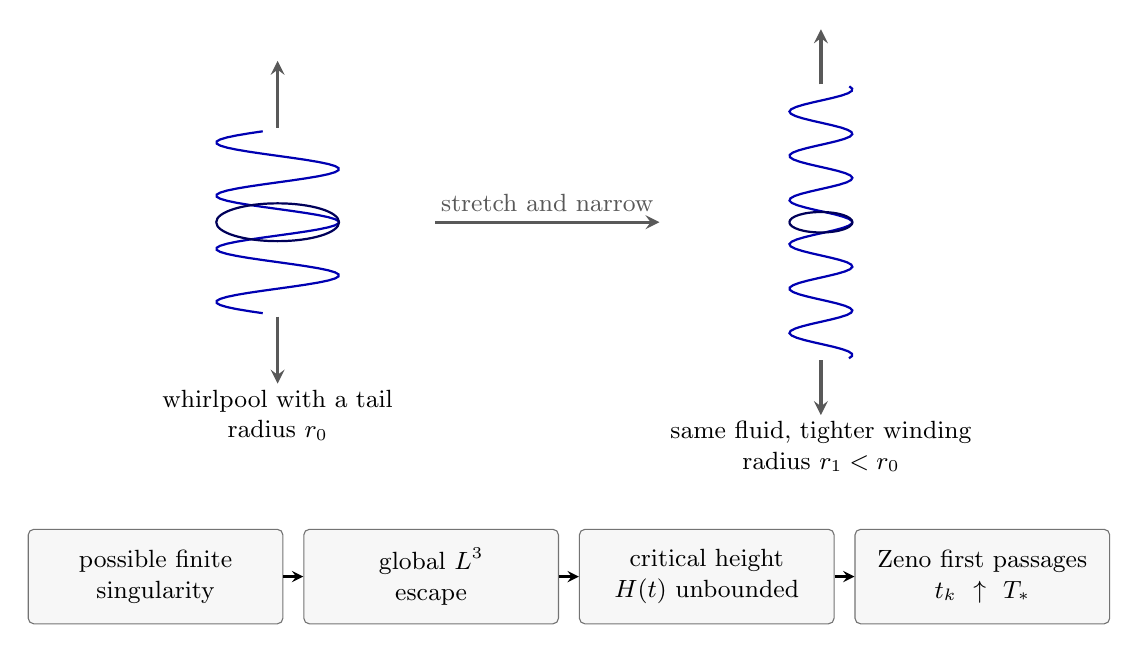
\begin{tikzpicture}[
  >=stealth,
  logic/.style={draw=black!55,rounded corners=2pt,fill=black!3,
    align=center,text width=3.0cm,minimum height=1.2cm,font=\small},
  note/.style={align=center,font=\small}
]
  \draw[blue!70!black,thick,domain=-1.1:1.1,samples=90]
    plot ({-3.7+0.78*cos(560*\x)},{1.05*\x+2.4});
  \draw[blue!35!black,thick]
    (-4.48,2.4) arc[start angle=180,end angle=540,x radius=.78,y radius=.24];
  \draw[->,very thick,black!65] (-3.7,3.6)--(-3.7,4.45);
  \draw[->,very thick,black!65] (-3.7,1.2)--(-3.7,.35);
  \node[note] at (-3.7,-.05) {whirlpool with a tail\\radius \(r_0\)};

  \draw[->,very thick,black!65]
    (-1.7,2.4)--(1.15,2.4)
    node[midway,above,note] {stretch and narrow};

  \draw[blue!70!black,thick,domain=-1.35:1.35,samples=120]
    plot ({3.2+0.40*cos(820*\x)},{1.28*\x+2.4});
  \draw[blue!35!black,thick]
    (2.80,2.4) arc[start angle=180,end angle=540,x radius=.40,y radius=.13];
  \draw[->,very thick,black!65] (3.2,4.15)--(3.2,4.85);
  \draw[->,very thick,black!65] (3.2,.65)--(3.2,-.05);
  \node[note] at (3.2,-.45) {same fluid, tighter winding\\radius \(r_1<r_0\)};

  \node[logic] (a) at (-5.25,-2.1) {possible finite\\singularity};
  \node[logic] (b) at (-1.75,-2.1) {global \(L^3\)\\escape};
  \node[logic] (c) at (1.75,-2.1) {critical height\\\(H(t)\) unbounded};
  \node[logic] (d) at (5.25,-2.1) {Zeno first passages\\\(t_k\uparrow T_*\)};
  \draw[->,thick] (a)--(b);
  \draw[->,thick] (b)--(c);
  \draw[->,thick] (c)--(d);
\end{tikzpicture}
\captionof{figure}{The perfectly stretching vortex keeps one physical danger in view while the implication chain below it moves to global quantities.}
\label{fig:BalancedVortexCriticalRoute}
\end{center}


This is the Zeno cascade.
The picture and the exact endpoint demand now sit beside each other.
The perfectly stretching vortex is the physical limit case; finite maximality would force the full field, whatever its local geometry, through infinitely many new critical-height levels before one finite time.
Becoming thinner is only one part of the demand.
The finite-time demand cannot stop at velocity.
If any fixed order of its time response stayed uniformly bounded, repeated integration would keep the velocity bounded too.
In physical language, the problem has passed from velocity to acceleration, from changing acceleration to jerk, and onward.
The singularity has opened a Tower.
